\documentclass{article}
\usepackage{graphicx} % new way of doing eps files
\usepackage{listings} % nice code layout
\usepackage[usenames]{color} % color
\definecolor{listinggray}{gray}{0.9}
\definecolor{graphgray}{gray}{0.7}
\definecolor{ans}{rgb}{1,0,0}
\definecolor{blue}{rgb}{0,0,1}
% \Verilog{title}{label}{file}
\newcommand{\Verilog}[3]{
  \lstset{language=Verilog}
  \lstset{backgroundcolor=\color{listinggray},rulecolor=\color{blue}}
  \lstset{linewidth=\textwidth}
  \lstset{commentstyle=\textit, stringstyle=\upshape,showspaces=false}
  \lstset{frame=tb}
  \lstinputlisting[caption={#1},label={#2}]{#3}
}


\author{Josh Young}
\title{Lab 5}

\begin{document}
\maketitle

\section{Introduction}
Lab 5 has the user begin implementation of the next stage for the mips machine, namely, the decoding stage. The lab walks the user through creating and testing 2 parts of the stage. These are the control unit and the sign extender. Once the two items were developed, simulations were ran in order to validate the code and insure there are no errors.

\section{Interface}
The sign extender is quite simple. The input is a 16 bit binary number, and the output is a 32 bit binary number where the most significant bit of the input is concatenated multiple times for the output. The control unit is slightly more complex; this is due to multiple outputs that are dependent on the opcode that the control is fed. The control unit has 8 outputs, which are RegDst, Branch, MemRead, MemtoReg, ALUOp, ALUSrc, and RegWrite. These outputs are either 0 or 1 with the exception of the ALUOp, which is a 2 bit code. 

\section{Design}
The sign extender and control are an invaluable part of the decoding stage.

\section{Implementation}
The code used for creating the sign extender can be seen in Listing~\ref{code:sign} on page~\pageref{code:sign}. The code for creating the control can be seen in Listing~\ref{code:control} on page~\pageref{code:control}.

\Verilog{Verilog code for implementing a sign extender.}{code:sign}{../code/2_decode/sign_extender.v}

\Verilog{Verilog code for implementing the control.}{code:control}{../code/2_decode/control.v}

\section{Test Bench Design}
The lab had the user create two test benches, one for the control unit, and the other for the sign extender. The goal for the test bench was to try and 'break' the code for the control unit or sign extender. For the sign extender, this was done by feeding the input different binary numbers and observe if the sign of the number was correctly extended for all 32 bits. As for the control, a series of actual opcodes (i.e. for branch, load, store) as well as made up ones where dumped into the input. 

The verilog code for the sign extender test bench can be viewed in Listing~\ref{code:SignTest} on page~\pageref{code:SignTest}, and the code for the control test may be viewed in Listing~\ref{code:Controltest} on page~\pageref{code:Controltest}.

\Verilog{Verilog code for testing the sign extender.}{code:SignTest}{../code/2_decode/sign_ext_test.v}

\Verilog{Verilog code for testing the control.}{code:Controltest}{../code/2_decode/control_test.v}

\section{Simulation}
By viewing the timing diagrams for the control and sign extender, one can see that both behave as expected. The timing diagram for the control can be viewed in Figure~\ref{fig:control_test}. The timing diagram for the sign extender may be viewed in Figure~\ref{fig:sign_extend_test}.



\section{Conclusions}
The goal for Lab 5 was to create and test 2 components of the decoding stage, namely, the sign extender, and the control. The control is used to get information based off of the corresponding opcode that was fed to the input, and the sign extender simply extends the most significant bit of a 16 bit binary number and turns it into a 32 bit number with the same value. The test benches for each of the devices show that they are both in working order.

\begin{figure}
	\begin{center}
		\caption{Timing diagram for the control test.}\label{fig:control_test}
		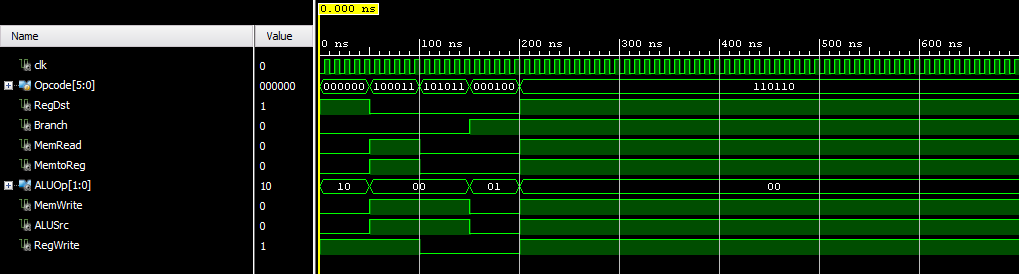
\includegraphics[width=0.9\textwidth]{../images/control_test.png}
	\end{center}
\end{figure}
\begin{figure}
	\begin{center}
		\caption{Timing diagram for the sign extender test.}\label{fig:sign_extend_test}
		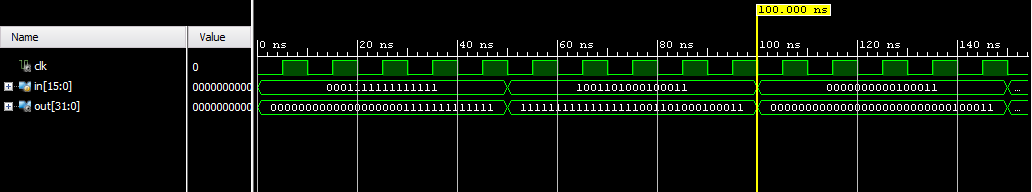
\includegraphics[width=0.9\textwidth]{../images/sign_extend_test.png}
	\end{center}
\end{figure}
\end{document} 
